\documentclass{article}
\usepackage[utf8]{inputenc}

\title{Laboratorio01U2_INTELIGENCIA_NEGOCIOS}
\author{edwartbalcon}
\date{Septiembre 2021}

\usepackage[utf8]{inputenc}
\usepackage[spanish]{babel}
\usepackage{natbib}
\usepackage{graphicx}

\begin{document}

\title{Caratula}

\begin{titlepage}
\begin{center}
\begin{Large}
\textbf{UNIVERSIDAD PRIVADA DE TACNA} \\
\end{Large}
\vspace*{-0.025in}
\begin{figure}[htb]
\begin{center}

\includegraphics[width=6cm]{./images/logo_UPT}
\end{center}
\end{figure}
\vspace*{-0.025in}
\begin{Large}
\textbf{FACULTAD DE INGENIERIA} \\
\end{Large}
\vspace*{0.05in}
\begin{Large}
\textbf{Escuela Profesional de Ingeniería de Sistema} \\
\end{Large}


\vspace*{0.4in}

\vspace*{0.1in}
\begin{Large}
\textbf{Informe de laboratorio 04: Crear una Dimensión Regular con SQL
Server Analysis Services} \\
\end{Large}

\vspace*{0.3in}
\begin{Large}
\textbf{Curso: Inteligencia de negocios} \\
\end{Large}

\vspace*{0.3in}
\begin{Large}
\textbf{DOCENTE: Ing. Patrick Cuadros Quiroga} \\
\end{Large}

\vspace*{0.2in}
\vspace*{0.1in}
\begin{large}

\begin{Large}
\textbf{Alumno: Balcon Coahila, Edwart Juan\hfill	(2013046516) } \\
\end{Large}

\vspace*{0.15in}
\begin{Large}
\textbf{Tacna – Perú} \\
\end{Large}

\vspace*{0.05in}
\begin{Large}
\textbf{2021 } \\
\end{Large}

\end{large}
\end{center}

\end{titlepage}

%%INICIO Resumen
\section{Onjetivos}
Crear una Dimensión sobre un Cubo Multidimensional en SQL Server Analysis Services para que usuarios
finales puedan explotar la información.
%%FIN Resumen

%%INICIO Resumen
\section{Dimension Regular }
Las dimensiones regulares representan datos descriptivos que proporcionan contexto para datos modelados en dimensiones de medida. Una dimensión regular se divide en grupos de información denominados niveles. A su vez, los distintos niveles se pueden organizar en jerarquías. Por ejemplo, la dimensión de un producto puede contener los niveles Product Line, Product Type y Product organizados en una única jerarquía denominada Product. Otro ejemplo es una dimensión de tiempo que tiene los niveles Year, Quarter, Month, Week y Day, organizados en dos jerarquías. La primera jerarquía YQMD contiene los niveles Year, Quarter, Month y Day, la otra jerarquía YWD contiene los niveles Year, Week y Day.
\\
\\
La definición más sencilla de un nivel consta de una clave de empresa y un título, donde cada uno de estos elementos hace referencia a un elemento de consulta. Una instancia (o fila) de un nivel se define como miembro de ese nivel. Se identifica por un nombre exclusivo de miembro, que contiene los valores de las claves de empresa de los niveles actual y superior. Por ejemplo, [gosales].[Products].[ProductsOrg].[Product]->[All Products].[1].[1].[2] identifica un miembro que se encuentra en el cuarto nivel, Product, de la jerarquía ProductsOrg de la dimensión [Products] que está en el espacio de nombres [gosales]. El título para este producto es TrailChef Canteen, que es el nombre que aparece en el árbol de metadatos y en el informe.
\\
\\
El nivel se puede definir como exclusivo si la clave de empresa es suficiente para identificar cada conjunto de datos para un nivel. En el modelo Great Outdoors Sales, los miembros del nivel Product no necesitan la definición de tipo Product porque muchos tipos de producto diferentes no tienen números de producto asignados. Un nivel que no está definido como exclusivo es similar a un determinante que utiliza claves de varias partes porque se necesitan claves de niveles superiores de granularidad. Consulte: Utilización de determinantes con claves de varias partes. Si miembros de los miembros ancestro no son exclusivos pero el nivel se ha identificado como exclusivo, los datos para los miembros no exclusivos se informan como un único miembro. Por ejemplo, si City se define como exclusivo y se identifica por el nombre, los datos para London, England y London, Canada, se combinarán.
%%FIN Resumen

%%----------------------------------------------------------------------------------------------------------------------------------------------------------
%%INICIO Marco Teórico
\section{Procedimiento}

Tomando como base el laboratorio anterior se construyo un cubo básico Multidimensional, pero se tenia
dificultad al momento de explotar la información. Este detalle se debe a que no tuvimos un manejo más
personalizado de los atributos de las dimensiones. En este laboratorio se abordará como crear y configurar
una dimensión regular en Analysis Services.

\section{Creación de una Dimensión Regular}  

1. En el Solution Explorer nos ubicamos en Data Sources View y podemos ver que tenemos la vista de las
siguientes tablas:
	\begin{center}
	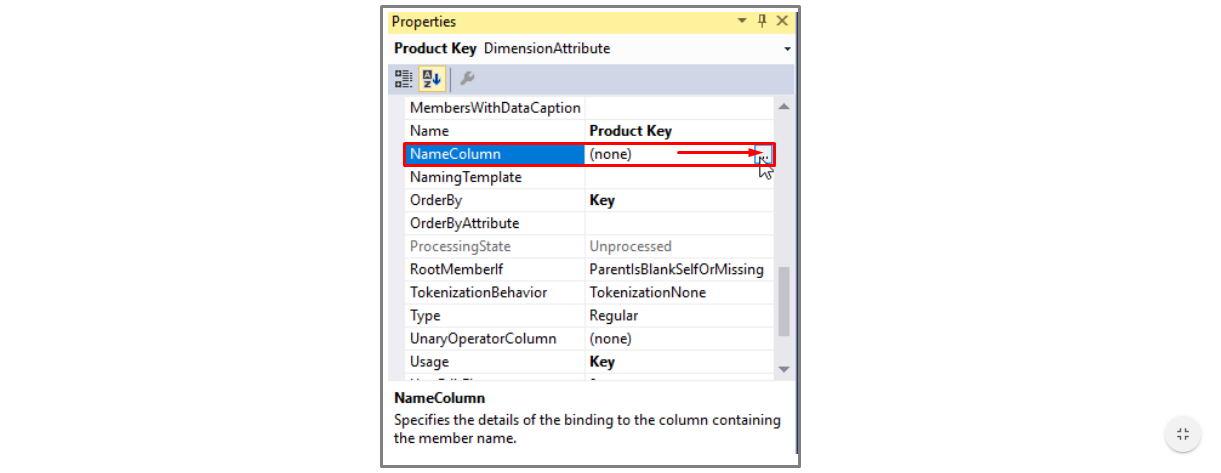
\includegraphics[width=\columnwidth]{images/task1/img1}
	\end{center}	


2. Siempre se recomienda primero crear las dimensiones y como paso final recién crear el cubo, es por eso que
eliminamos el cubo creado en el primer post. Luego nos dirigimos a Dimensions. Click derecho y ubicamos
New Dimension
	\begin{center}
	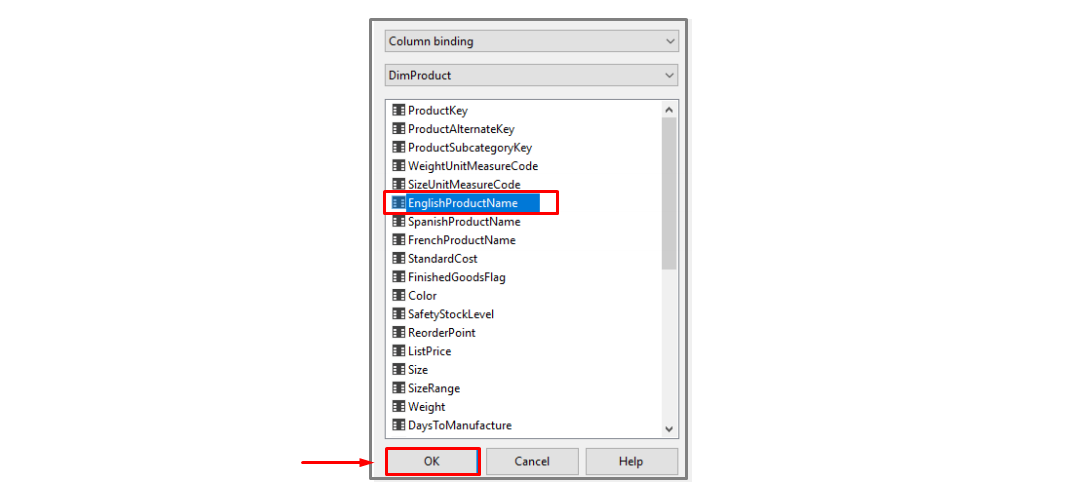
\includegraphics[width=\columnwidth]{images/task1/img2}
	\end{center}	

3. Nos abrirá un Wizard, donde la primera ventana es un resumen de lo que se puede realizar.
	\begin{center}
	
\includegraphics[width=\columnwidth]{images/task1/img3}
	\end{center}	

4. Click en Next.
Esta paso en el wizard es muy importante ya que nos permite seleccionar el origen de la dimensión a crear.
Se tienen 4 opciones:
			\begin{itemize}
				\item Use an existing table: Se seleccionará alguna tabla perteneciente al Data Source View.
				\item Generate a time table in the data source: Crea una tabla en el data source, pero esta nueva tabla no
es replicada en el origen.
\item Generate a time table in the server: Crea una tabla en el server, y esta nueva tabla es replicada en
el origen.
\item Generate a non table in the data source: Crea una tabla en el data source a partir de unos
Templates que tiene el Data Tools.

Seleccionamos la primera opcion:

			\end{itemize}

	\begin{center}
	
\includegraphics[width=\columnwidth]{images/task1/img4}
    \end{center}	

5. Click en Next.
Seleccionamos el Data source view (podríamos tener más de uno) y la tabla Dimensión, en este ejemplo
DimProduct. En Key columns por defecto siempre selecciona al Primary Key de la tabla, pero este valor luego
podría ser cambiado. También podemos añadirle un Name Column a este Key column pero lo dejaremos tal
como esta:
    
	\begin{center}
	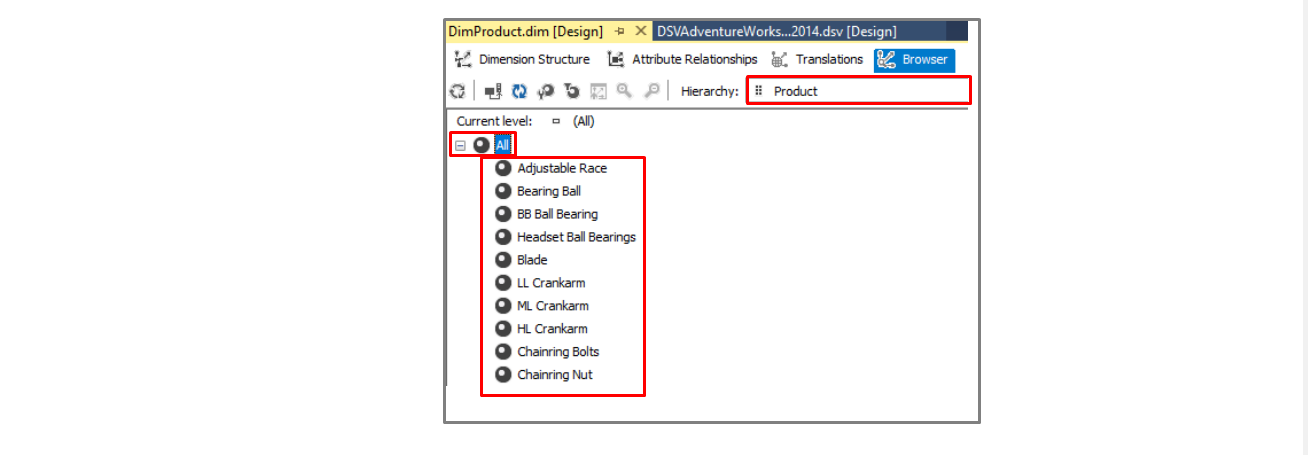
\includegraphics[width=\columnwidth]{images/task1/img5}
    \end{center}	

6. Click en Next.
Marcamos los atributos con los cuales trabajaremos:
    
	\begin{center}
	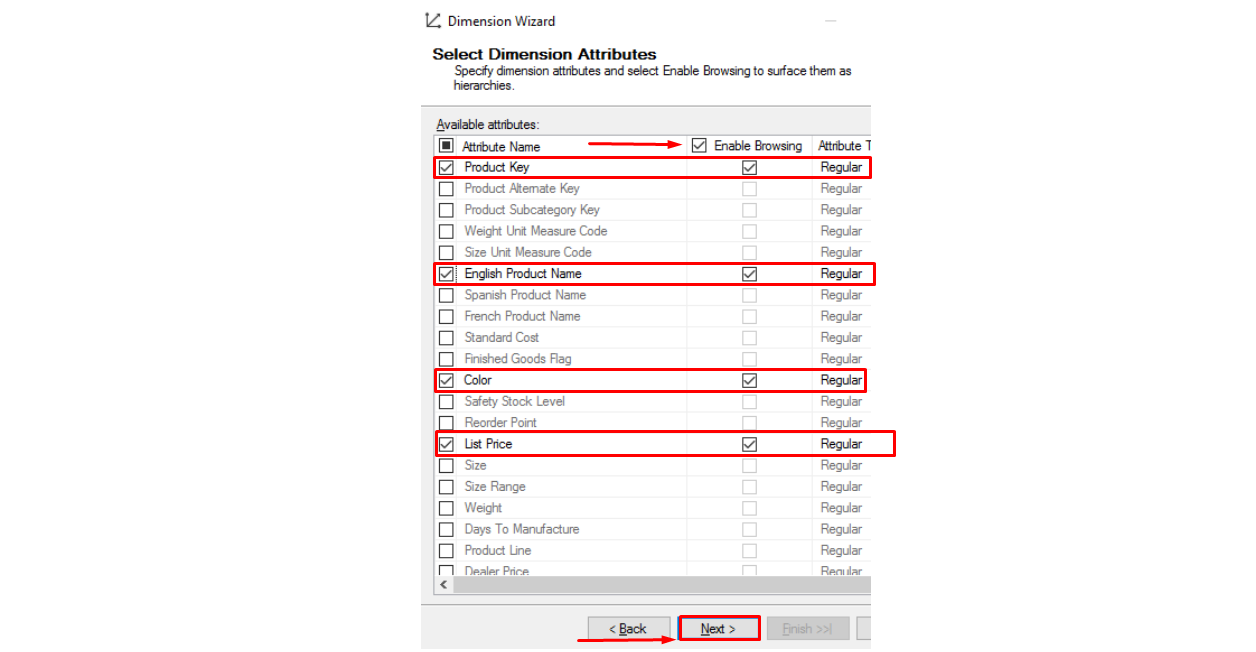
\includegraphics[width=\columnwidth]{images/task1/img6}
    \end{center}	

7. Click en Next.
Indicamos el Nombre a la dimensión:
    
	\begin{center}
	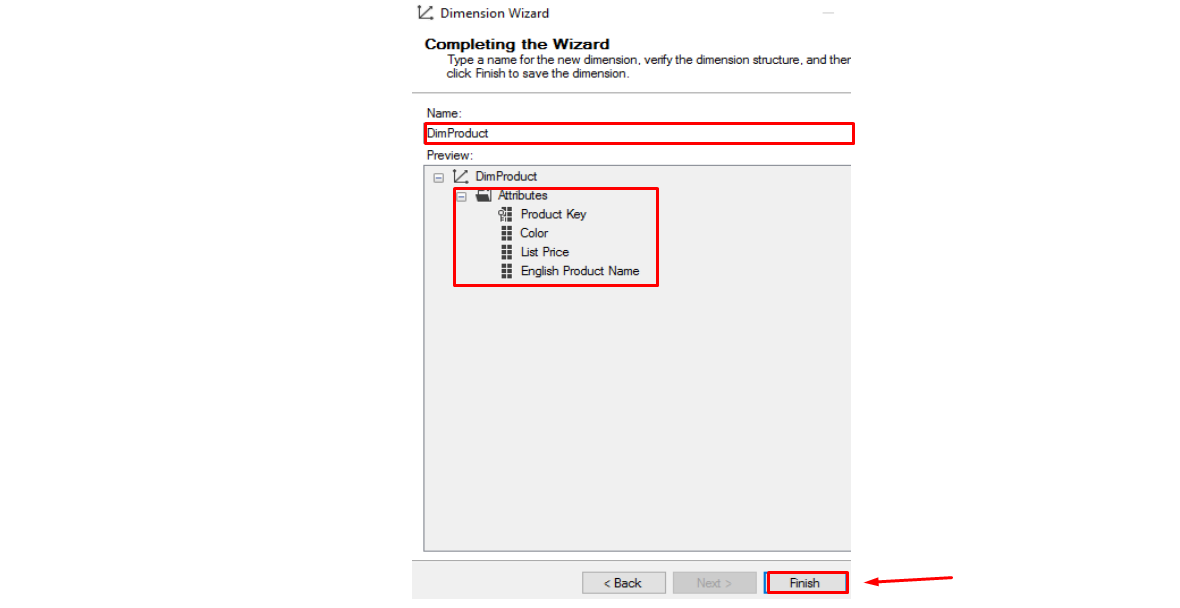
\includegraphics[width=\columnwidth]{images/task1/img7}
    \end{center}	

Click en Finish.

    
\section{Procesar una Dimensión} 

1. Ya creada la dimensión, el siguiente paso es Procesarla para ver la generación de los datos. En la pestaña
de Dimension Structure ubicamos la opción de Process:

	\begin{center}
	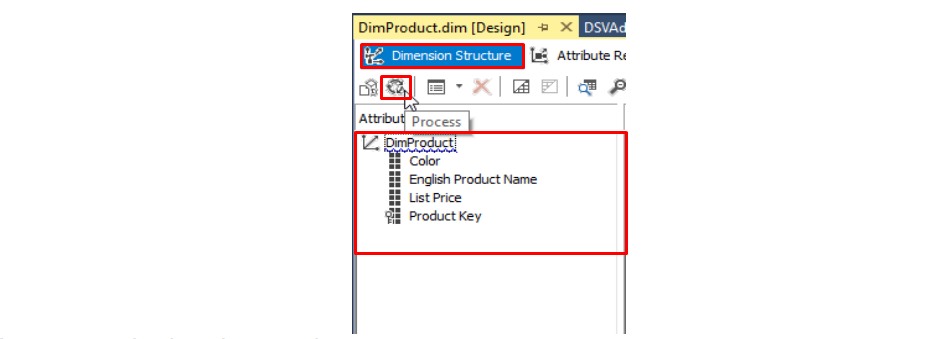
\includegraphics[width=\columnwidth]{images/task2/img13}
	\end{center}	

2. Nos mostrará un mensaje de advertencia:

	\begin{center}
	
\includegraphics[width=\columnwidth]{images/task2/img14}
    \end{center}	
    
Click en Yes.

3. Luego Click en Run…
Se nos abrirá una ventana donde nos mostrará el progreso del proceso de la dimensión DimProduct:
	\begin{center}
	
\includegraphics[width=\columnwidth]{images/task2/img17}
    \end{center}	
    

4. En la pestaña de Browser exploramos los atributos y los valores que contienen.
Exploramos el atributo Color:

	\begin{center}
	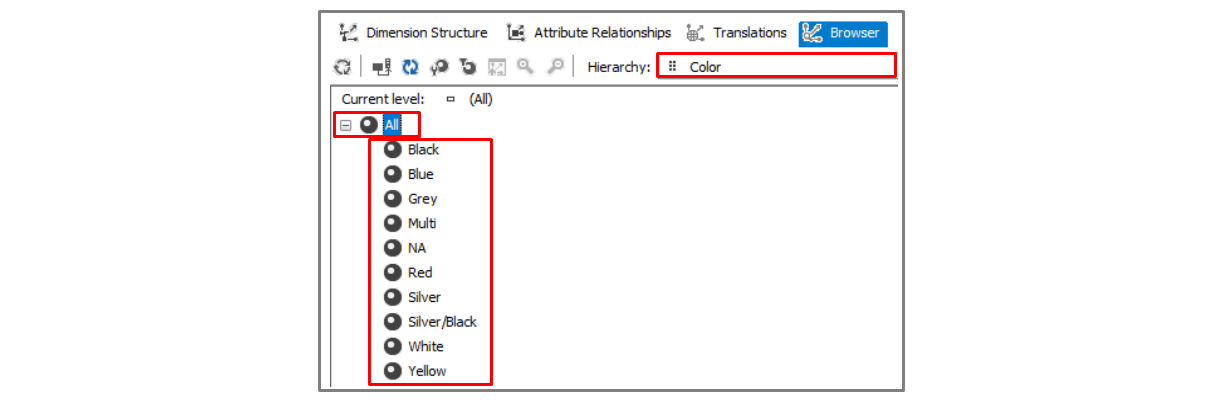
\includegraphics[width=\columnwidth]{images/task2/img19}
    \end{center}	
    
5. Exploramos el atributo English Product Name:
    \begin{center}
	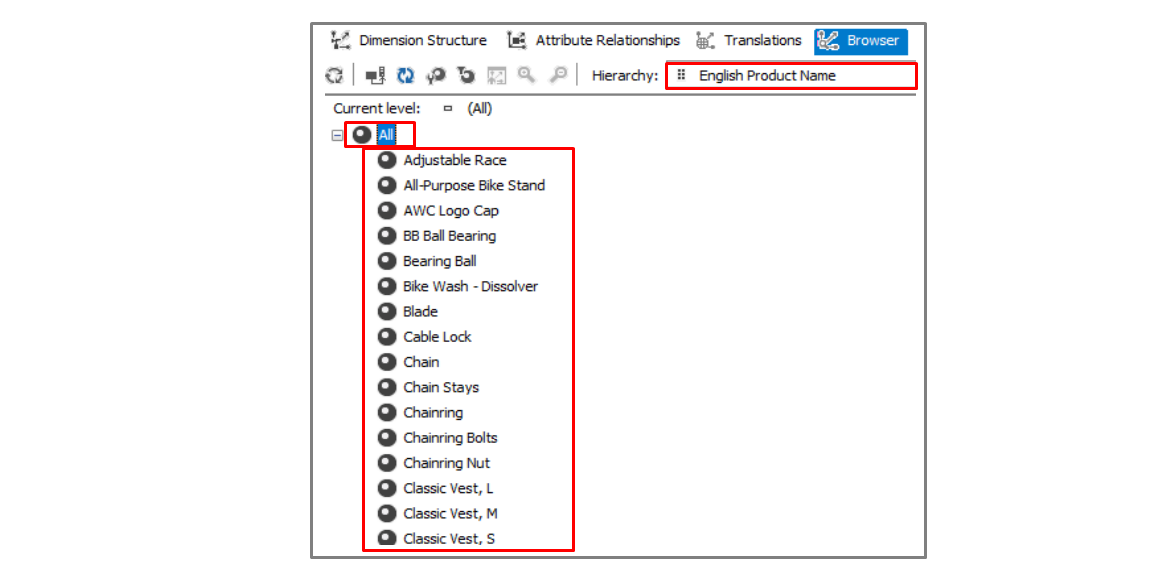
\includegraphics[width=\columnwidth]{images/task2/img21}
    \end{center}	
 
6. Exploramos el atributo Product Key:

	\begin{center}
	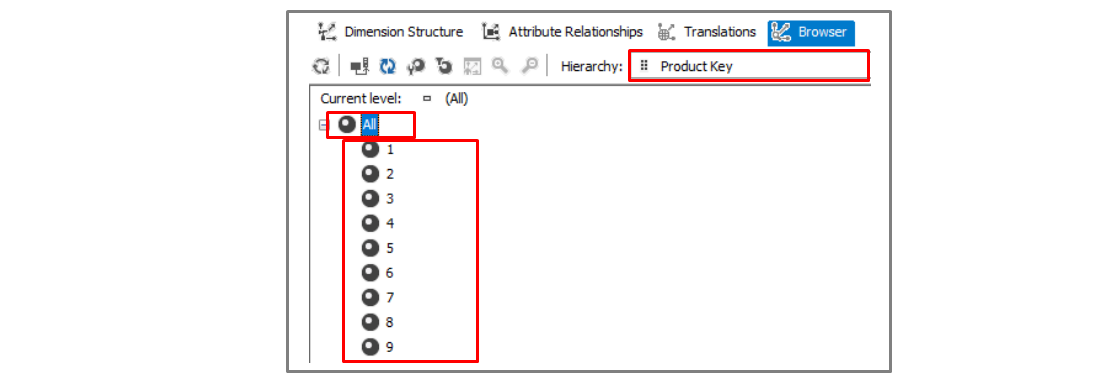
\includegraphics[width=\columnwidth]{images/task2/img22}
    \end{center}	
   
Es aquí donde detectamos que si bien es cierto nos muestra los valores de Product Key , lo recomendable
es que este atributo no sea visible para el usuario final, ya que esta es una llave propia del DW.
	
\section{Configurar el Name Column en una Dimensión}  

1. En las propiedades del atributo Product Key nos ubicamos en NameColumn:

	\begin{center}
	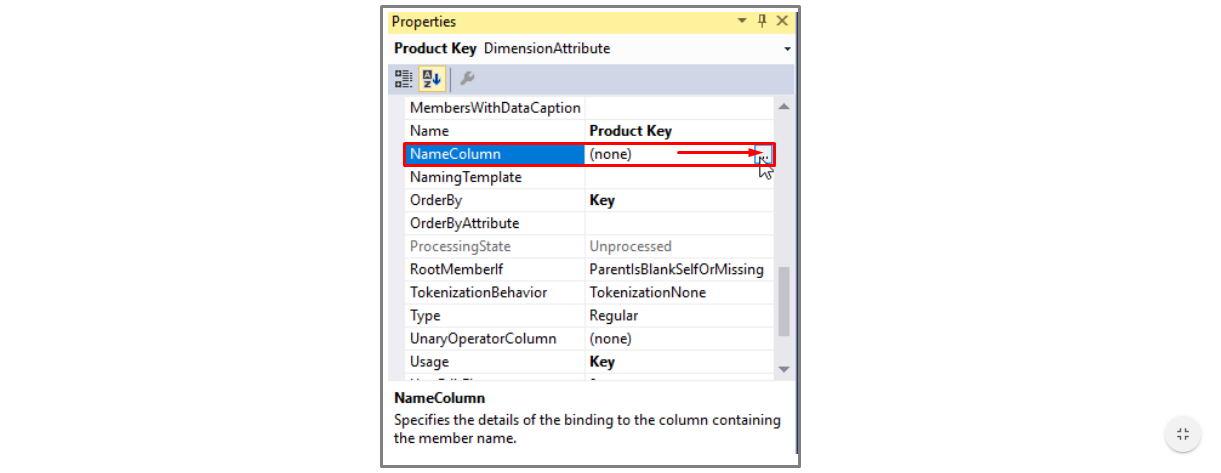
\includegraphics[width=\columnwidth]{images/task1/img1}
	\end{center}	


2. Nos abrirá una ventana donde podemos enmascarar este atributo por otro, en este caso seleccionaremos el
atributo EnglishProductName:

	\begin{center}
	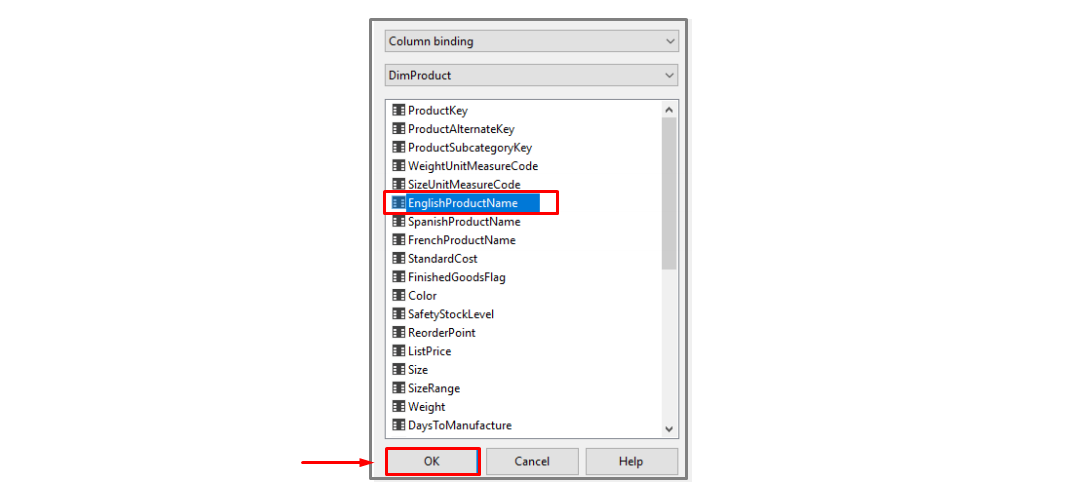
\includegraphics[width=\columnwidth]{images/task1/img2}
	\end{center}	

Click en Ok.

3. Eliminaremos el atributo EnglishProductName y renombraremos el atributo Product Key por Product:

	\begin{center}
	
\includegraphics[width=\columnwidth]{images/task1/img3}
	\end{center}	

Procesamos la dimensión DimProduct.

4. Una vez procesada la dimensión nos volvemos a Reconcetar al mismo:

	\begin{center}
	
\includegraphics[width=\columnwidth]{images/task1/img4}
    \end{center}	

5. Si ahora consultamos el atributo Product obtendremos lo siguiente:

	\begin{center}
	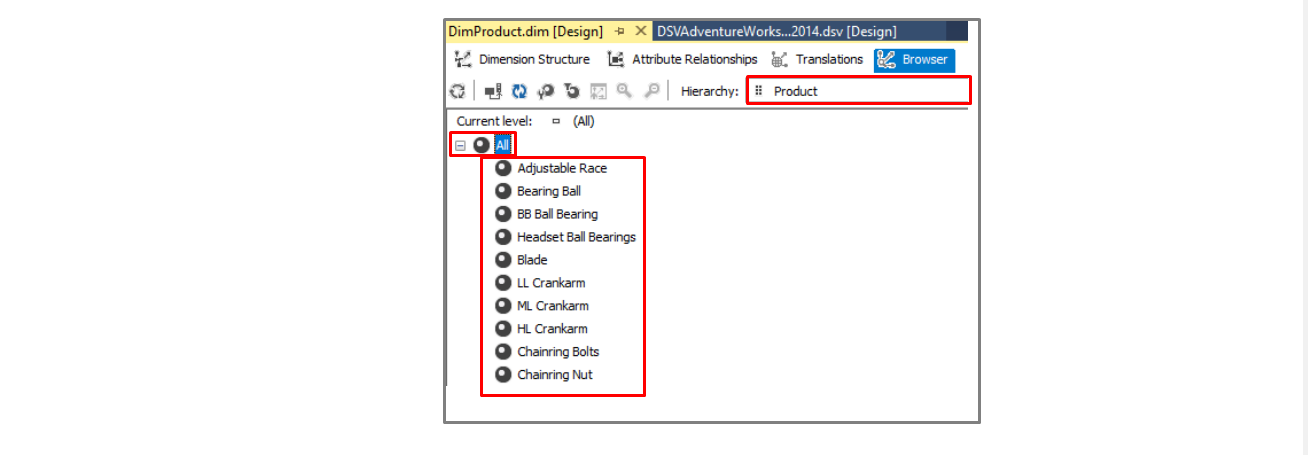
\includegraphics[width=\columnwidth]{images/task1/img5}
    \end{center}	


    


\end{document}